\section{Lab Tasks: Defense}
%
\subsection{Task 4: Enabling Elgg's Countermeasure}
%
\begin{figure}
    \centering
    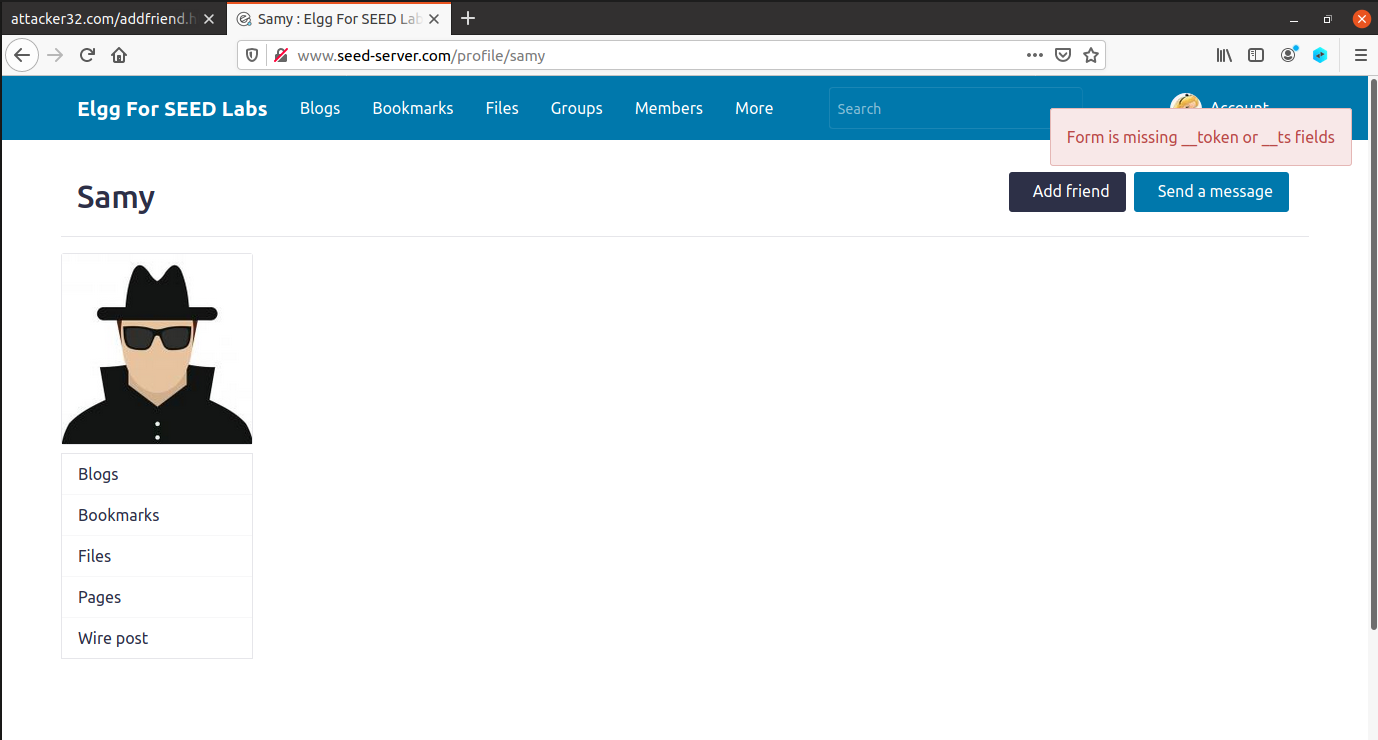
\includegraphics[height=\textheight,width=\textwidth,keepaspectratio]
    {figures/add_friend_countermeasure.png}
    \caption{CSRF countermeasure prevents the HTTP GET request forging attack.}
    \label{fig:counter_add_friend}
\end{figure}

\begin{figure}
    \centering
    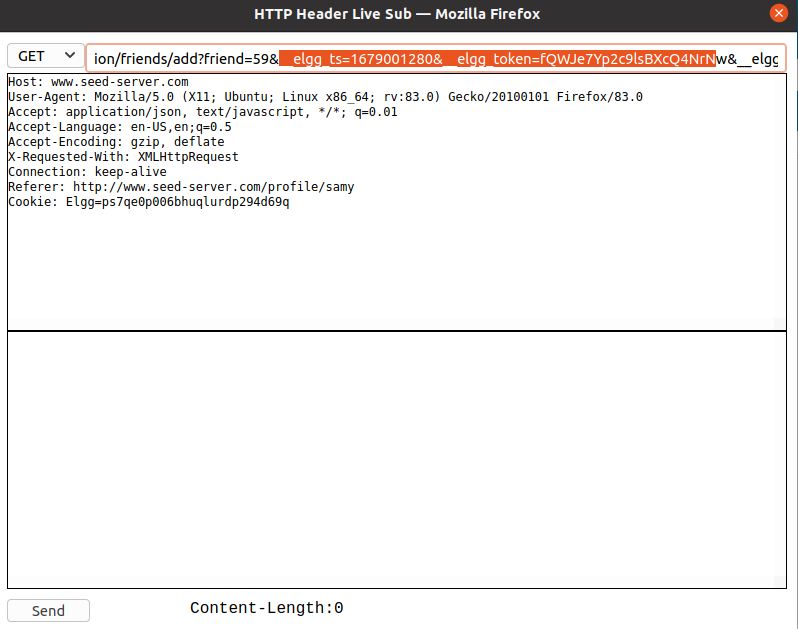
\includegraphics[height=\textheight,width=\textwidth,keepaspectratio]
    {figures/token_http_get.png}
    \caption{Secret tokens embedded in URL of an HTTP GET request.}
    \label{fig:secret_token}
\end{figure}

\begin{figure}
    \centering
    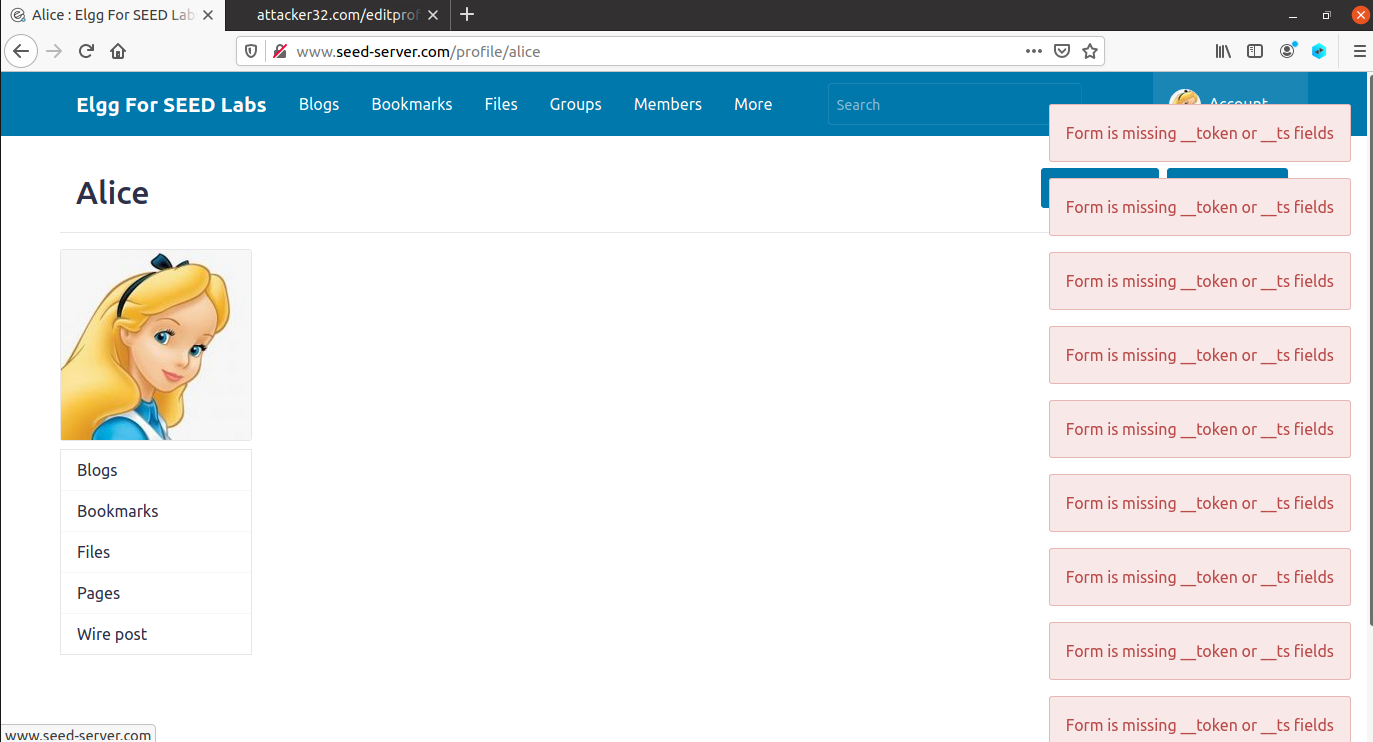
\includegraphics[height=\textheight,width=\textwidth,keepaspectratio]
    {figures/edit_profile_countermeasure.png}
    \caption{CSRF countermeasure prevents the HTTP POST request forging attack.}
    \label{fig:counter_edit_profile}
\end{figure}

After turn on the CSRF countermeasure by commenting out the {\fontfamily{qcr}\selectfont
return} line, it turned out that we cannot do CSRF attacks like above. For instance,
when we conducted the {\fontfamily{qcr}\selectfont add\_friend} attack, Elgg page raised
an alert noticing that {\fontfamily{qcr}\selectfont \_\_elgg\_token} and
{\fontfamily{qcr}\selectfont \_\_elgg\_ts} fields are missing
(see \autoref{fig:counter_add_friend}). In the case of {\fontfamily{qcr}\selectfont edit\_profile}
attack, as the attacker's page is reloaded, the forged POST request is re-triggered, so
a chain of red alerts was shown (see \autoref{fig:counter_edit_profile}).

Logged-in as Alice and then pressed the {\fontfamily{qcr}\selectfont Add friend} button,
we captured a HTTP GET request including two secret tokens (see \autoref{fig:secret_token}).

\begin{itemize}
    \item \_\_elgg\_ts: 1679001280
    \item \_\_elgg\_token: fQWJe7Yp2c9lsBXcQ4NrNw
\end{itemize}

The attacker cannot send these secret tokens as he does not know their values.
The access control system of browser does not allow the JavaScript code in the
malicious webpage access any content in Elgg's pages. In addition, as secret
tokens are hashed value of \emph{site secret value, timestamp, user session ID,
and random generated session string}, it is nearly impossible to guess. On the
other hand, if the attacker wants to do brute-force based on the hash collision,
he has to wait in a long time. Meanwhile, these two secret values have changed
periodcally or once the user starts a new session. So if the attacker can
brute-force these two hash values, these finding won't be valid anymore.
